\documentclass{article}

\PassOptionsToPackage{numbers, compress}{natbib}
\usepackage[final]{neurips_2019}

\usepackage[utf8]{inputenc}
\usepackage[T1]{fontenc}
\usepackage{hyperref}
\usepackage{url}
\usepackage{booktabs}
\usepackage{amsfonts}
\usepackage{nicefrac}
\usepackage{microtype}
\usepackage{amsmath,amssymb,bm}
\usepackage{graphicx}
\usepackage{xcolor}
\usepackage{tikz}
\usetikzlibrary{positioning,arrows.meta,calc}

\newcommand{\R}{\mathbb{R}}

\title{Does the Gate Listen? Reproducing and Extending GS-Fuse\\ for Event-Driven Financial Forecasting}

\author{%
  [Member 1] \And [Member 2] \And [Member 3] \And [Member 4] \\
  Carnegie Mellon University, Pittsburgh, PA 15213 \\
  \texttt{\{andrew-id1, andrew-id2, andrew-id3, andrew-id4\}@andrew.cmu.edu}
}

\begin{document}

\maketitle

% =====================================================================
\begin{abstract}
GS-Fuse (KDD'26) fuses a frozen time-series foundation model with a frozen LLM through a gate supervised by a Granger-style signal: the gate should open for event text when the text reduces forecast error.
We reproduce GS-Fuse on the 2008--2024 S\&P~500 macro-event benchmark (11{,}647 events, 5-minute bars, 140-step horizon) and add two fusion extensions, a mixture-of-experts (MoE) gate and a BLIP-2-style Q-Former.
Our reproduction reaches a test MSE of $6.33\times10^{-4}$, 2.1\% below persistence and 5\% below an independent team run, and caching the frozen LLM cuts training of all variants from an estimated 48\,h to 10\,h.
The analysis exposes two problems: the text gate is almost constant ($0.524\pm0.003$), and the released split places 90.7\% of test events on exactly the same price window as some training event.
The Q-Former nearly triples the gain from text (0.5\%$\to$1.4\%) but no variant lowers overall error yet.
We propose a leakage-free protocol, a biologically inspired surprise-gated memory, and a memristor-based analog expert layer as next steps.
\end{abstract}

% =====================================================================
\section{Motivation and objectives}
Scheduled releases (CPI, payrolls, FOMC) and news are the main exogenous shocks for intraday equity prices. A forecaster that reads them should beat a price-only model \emph{when} the text is informative and ignore it otherwise. GS-Fuse~\cite{gsfuse} implements this with a gate trained to open in proportion to how much the text helps. We ask whether the gate behaves as intended and whether stronger fusion operators help.
\textbf{(O1, quantitative)} Reproduce GS-Fuse at full scale and beat persistence and an independent team run (test MSE $6.66\times10^{-4}$).
\textbf{(O2, quantitative)} Compare three fusion variants under identical data and budget on MSE/MAE at horizons $H\in\{35,70,140\}$ and on endpoint directional hit rate (DHR).
\textbf{(O3, qualitative)} Determine whether the gate is event-aware: does text openness vary with event type and with the measured benefit of the text?

% =====================================================================
\section{Related work and background}
\textbf{Event-driven forecasting.} CAMEF~\cite{camef} introduced our benchmark and fuses LLM embeddings of macro releases with price windows, using LLM-generated counterfactual rewrites. GS-Fuse~\cite{gsfuse} adds a frozen MOMENT~\cite{moment} encoder, bidirectional cross-attention with InfoNCE alignment~\cite{cpc}, and a Granger-supervised gate: text ``Granger-causes'' the target~\cite{granger} if adding it lowers error, and this error reduction is the gate's target. \emph{Gap:} neither paper shows whether the gate varies across events or reports a text-free control on the same samples.
\textbf{LLMs for time series.} Time-LLM~\cite{timellm} and TimeCMA~\cite{timecma} use text as a prompt \emph{about} the series rather than as an exogenous event, and do not gate modalities per sample.
\textbf{Fusion operators.} Sparse MoE layers~\cite{shazeer2017,switch} route heterogeneous inputs to specialized experts; BLIP-2's Q-Former~\cite{blip2} compresses long sequences from a frozen encoder into a few learned queries. Both motivate our extensions.
\textbf{Background on metrics and baselines.} MSE/MAE are the standard point-forecast errors~\cite{hyndman}; directional accuracy must be judged against its base rate~\cite{pesaran}. Since prices are close to a random walk~\cite{fama}, \emph{persistence} (repeat the last price) is the natural bar for MSE and ``always up'' for DHR, and simple baselines often beat complex transformers~\cite{dlinear}; we therefore score them on exactly the same samples as our models.

% =====================================================================
\section{Proposed solution}
We keep the GS-Fuse encoders, losses and three-stage schedule and replace only the fusion block (Figure~\ref{fig:arch}).
\textbf{MoE gate:} $K=4$ expert gates with top-2 routing; \emph{expected advantage:} official releases and noisy news can receive different text weights instead of one averaged gate.
\textbf{Q-Former:} 16 learned queries, conditioned on the market state, replace token-level cross-attention over $\sim$1{,}000 text tokens; \emph{expected advantage:} a fixed-size bottleneck that filters long reports and lets the price context choose what to read.
\textbf{Engineering:} the LLM runs under \texttt{no\_grad}, so we cache its embeddings, removing the $\sim$20\,s/step text-encoding cost.

% =====================================================================
\section{Model description}
\begin{figure}[t]
\centering
\resizebox{\linewidth}{!}{%
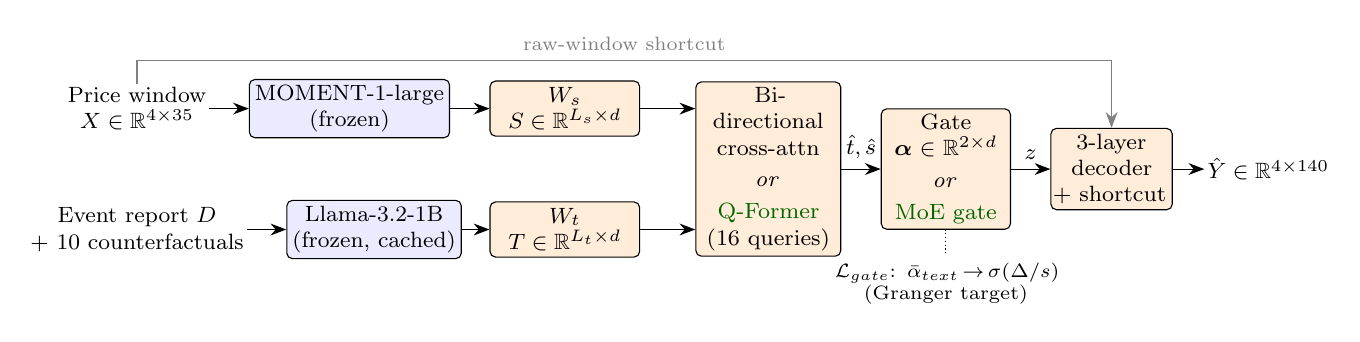
\begin{tikzpicture}[
  font=\footnotesize, >={Stealth[length=2mm]},
  box/.style={draw, rounded corners=2pt, align=center, minimum height=7mm, inner sep=2pt},
  frz/.style={box, fill=blue!8},
  trn/.style={box, fill=orange!15},
  io/.style={align=center, inner sep=1pt}]
\node[io] (x) {Price window\\$X\in\R^{4\times35}$};
\node[io, below=9mm of x] (d) {Event report $D$\\+ 10 counterfactuals};
\node[frz, right=5mm of x] (mo) {MOMENT-1-large\\(frozen)};
\node[frz, right=5mm of d] (ll) {Llama-3.2-1B\\(frozen, cached)};
\node[trn, right=5mm of mo, minimum width=19mm] (ps) {$W_s$\\$S\in\R^{L_s\times d}$};
\node[trn, minimum width=19mm] (pt) at (ps |- ll) {$W_t$\\$T\in\R^{L_t\times d}$};
\node[trn, anchor=west, minimum height=21mm, text width=17mm] (ca) at ($(ps.east)!0.5!(pt.east)+(7mm,0)$) {Bi-directional\\cross-attn\\[2pt]\textit{or}\\[2pt]\textcolor{green!40!black}{Q-Former}\\(16 queries)};
\node[trn, right=5mm of ca, text width=15mm] (g) {Gate $\bm\alpha\in\R^{2\times d}$\\[2pt]\textit{or}\\[2pt]\textcolor{green!40!black}{MoE gate}};
\node[trn, right=5mm of g, text width=14mm] (dec) {3-layer\\decoder\\+ shortcut};
\node[io, right=4mm of dec] (y) {$\hat Y\in\R^{4\times140}$};
\draw[->] (x) -- (mo); \draw[->] (d) -- (ll);
\draw[->] (mo) -- (ps); \draw[->] (ll) -- (pt);
\draw[->] (ps) -- (ca.west|-ps); \draw[->] (pt) -- (ca.west|-pt);
\draw[->] (ca) -- node[above]{$\hat t,\hat s$} (g);
\draw[->] (g) -- node[above]{$z$} (dec);
\draw[->] (dec) -- (y);
\draw[->, gray] (x.north) -- ++(0,3mm) -| node[pos=0.25, above]{\scriptsize raw-window shortcut} (dec.north);
\node[below=3mm of g, align=center, text width=30mm, font=\scriptsize] (gl) {$\mathcal{L}_{gate}$: $\bar\alpha_{text}\!\to\!\sigma(\Delta/s)$\\ (Granger target)};
\draw[densely dotted] (gl) -- (g);
\end{tikzpicture}}
\caption{Pipeline from raw data to forecast. Blue: frozen; orange: trained; green: our drop-in extensions.}
\label{fig:arch}
\end{figure}

\textbf{Inputs/outputs.} For event $i$ we take the $L=35$ five-minute bars before it, $X_i\in\R^{4\times L}$ (open/high/low/close, z-scored with training statistics), and its report $D_i$; the target is the next $P=140$ bars $Y_i\in\R^{4\times P}$ ($\approx$2 trading days; $H=35$ and $70$ are prefixes, $\approx$3\,h and $\approx$1 day).
\textbf{Encoders.} MOMENT features are projected to tokens $S\in\R^{L_s\times d}$ ($d=1024$) plus an instance vector $s$; Llama-3.2-1B~\cite{llama3} encodes 500-token windows (stride 400), mean-pooled and projected to $T\in\R^{L_t\times d}$.
\textbf{Fusion.} With multi-head attention $\mathrm{MHA}(Q,K,V)$, $H_t = T + \mathrm{MHA}(T,S,S)$ and $H_s = S + \mathrm{MHA}(S,T,T)$; $\hat t=\mathrm{LN}(\overline{H_t})$ and $\hat s=\mathrm{LN}(\overline{H_s}+s-\overline{S})$ are $\ell_2$-normalized ($\overline{\cdot}$: token mean, LN: layer norm). The gate is a softmax over the modality axis $m$ with temperature $\tau=1$:
\begin{equation}
\bm\alpha=\mathrm{softmax}_{m}\big(W_g[\hat t;\hat s]/\tau\big)\in\R^{2\times d},\qquad z=\bm\alpha_{1}\odot\hat t+\bm\alpha_{2}\odot\hat s .
\end{equation}
A 3-layer transformer decoder reads $z$ through 140 learned horizon queries; a linear shortcut on $\mathrm{vec}(X)$ is added to give $\hat Y$.
\textbf{MoE gate (ours).} Router probabilities $\pi=\mathrm{softmax}(R([\hat t;\hat s]))\in\R^{K}$ are kept for the top-2 experts and renormalized to $\tilde\pi$; then $\bm\alpha=\sum_k\tilde\pi_k\,\mathrm{softmax}_m(E_k([\hat t;\hat s])/\tau)$, so all gate losses apply unchanged. A Switch load-balancing loss $\mathcal{L}_{bal}=K\sum_k f_kP_k$~\cite{switch} ($f_k$: share of samples whose top-1 expert is $k$; $P_k$: mean router probability) prevents collapse.
\textbf{Q-Former (ours).} $N_q=16$ queries $Q_0=Q+W_c s$ ($W_c$ zero-initialized) pass through two blocks of self-attention, cross-attention to $T$ and a feed-forward layer; the output $H_t\in\R^{16\times d}$ replaces the text tokens.
\textbf{Justification.} Frozen backbones keep the trained parameters small for 7k training events; the gate makes the use of text explicit; the Granger target ties it to the error reduction text actually provides; the shortcut keeps a strong price-only path, important for near-random-walk prices.

% =====================================================================
\section{Dataset}
We use the GS-Fuse release, which combines the CAMEF corpus~\cite{camef} with FNDPID price series: 331{,}256 five-minute S\&P~500 OHLC bars (2008--2024) and 11{,}647 events in 12 folders, six official releases (1 jobless claims, 2 payrolls, 3 GDP, 4 FOMC, 5 CPI, 6 PPI) and six news streams (7--12). Each event has an LLM summary, 10 counterfactual rewrites and 5 same-type reports from other dates (negatives).
\textbf{Preprocessing.} Text is read as UTF-8 ignoring invalid bytes; prices are z-scored per channel with training statistics; each event is aligned to the last bar at or before 08:30 of its date.
\textbf{Split.} The loader concatenates events folder by folder and cuts 60/20/20\% \emph{by position} (train:test:vali); we sorted the directory traversal to make it OS-independent. Each split thus contains different event types, all spanning 2008--2024 (Table~\ref{tab:split}).

\begin{table}[t]
\caption{Event-type composition of the positional split.}
\label{tab:split}
\centering\small
\begin{tabular}{lrl}
\toprule
Split & \#events & Event types (count) \\
\midrule
Train & 6{,}988 & claims 632, payrolls 196, GDP 71, news-10 1727, news-11 1744, news-12 2618 \\
Test  & 2{,}329 & GDP 123, FOMC 125, CPI 194, PPI 186, news-7 569, news-8 1132 \\
Vali  & 2{,}330 & news-8 92, news-9 2238 \\
\bottomrule
\end{tabular}
\end{table}

% =====================================================================
\section{Evaluation metrics and loss}
\textbf{Metrics.} In the normalized space, averaged over 4 channels and the first $H$ steps~\cite{hyndman}: $\mathrm{MSE}_H=\frac{1}{4H}\sum_{c,h\le H}(\hat y_{c,h}-y_{c,h})^2$, and $\mathrm{MAE}_H$ likewise with $|\cdot|$.
Endpoint \textbf{DHR} on close is $\frac1N\sum_i \mathbf{1}[\mathrm{sign}(\hat y_{i,H}-x_{i,L})=\mathrm{sign}(y_{i,H}-x_{i,L})]$, compared with the always-up base rate~\cite{pesaran}; \textbf{Sharpe}~\cite{sharpe} is $\sqrt{A/H}\,\mu/\sigma$ of the per-event P\&L $\mathrm{sign}(\hat y_{i,H}-x_{i,L})(y_{i,H}-x_{i,L})$ ($A$: bars per year).
\textbf{Loss (stage 3).} With per-sample MSE $e_{full}$ and $e_{ts}$ (with/without text), $\Delta=e_{ts}-e_{full}$, $s=\max(\overline{|\Delta|},10^{-6})$ and channel-mean text gate $\bar\alpha_{text}$,
\begin{equation}
\begin{aligned}
\mathcal{L}={}&\underbrace{0.7\,\mathrm{MSE}+0.3\,\mathrm{MAE}}_{\mathcal{L}_{fc}}
+\mathcal{L}_{trip}
+0.1\big(\bar\alpha_{text}-\sigma(\mathrm{clip}(\Delta/s,\pm6))\big)^2\\
&+0.1\,\mathcal{L}_{inv}+0.01\,\mathcal{H}(\bm\alpha)+0.01\,\mathcal{L}_{nce}+0.1\,e_{ts}\,[+0.01\,\mathcal{L}_{bal}],
\end{aligned}
\end{equation}
where $\mathcal{L}_{trip}$ is a cosine triplet loss~\cite{facenet} (margin 1) against the hardest of 10 counterfactual and 5 other-date reports, $\mathcal{L}_{inv}$ ties a report to its counterfactual, $\mathcal{H}$ is gate entropy, and $\mathcal{L}_{nce}$ is token-level InfoNCE~\cite{cpc}.
\textbf{Relation to optimization.} $\mathcal{L}_{fc}$ optimizes exactly the reported MSE/MAE, so they are primary; the third term is the Granger supervision; DHR and Sharpe are not optimized and test whether lower MSE yields usable direction.
\textbf{Training.} Stage 1 trains the TS path on all sliding windows, stage 2 the text path, stage 3 everything; 2 epochs each, batch 8, AdamW~\cite{adamw} (lr $10^{-4}/10^{-4}/10^{-5}$), warmup and cosine decay; the best stage-3 epoch is chosen on validation MSE.

% =====================================================================
\section{Experimental depth and iteration}
\subsection{Baseline}
\textbf{Choice.} GS-Fuse~\cite{gsfuse} is the most recent published model on this benchmark, its code is public, and its central claim (the Granger-supervised gate) is exactly what our extensions modify. We use Llama-3.2-1B in fp32 instead of a larger LLM to fit our budget.
\textbf{Performance.} The baseline beats persistence by 2.1\% and the team run by 5\% in test MSE (Table~\ref{tab:main}), but its MAE is slightly \emph{higher} than persistence (0.01105 vs.\ 0.01075 at $H=35$) and its DHR is below always-up at $H=70$ and $140$. Its Sharpe exceeds always-up (0.93 vs.\ 0.50 at $H=140$), i.e.\ it is right on larger moves, but repeated windows make this optimistic (Section~\ref{sec:disc}).
\textbf{Motivation for extensions.} Text adds only 0.5\% over TS-only and the gate is nearly constant (Table~\ref{tab:abl}), so the single softmax gate does not use event information.
\textbf{Difference from the team run.} It used a 10$\times$ coarser stage-1 stride, Llama-3.2-3B in 4-bit, and non-strict resumes; no run fixes seeds.

\subsection{Implemented extensions and reproduction evidence}
We implemented the MoE gate and Q-Former (\texttt{--gate-type moe}, \texttt{--fusion-type qformer}), a signature-guarded text-embedding cache, W\&B logging of all stages and ablations, an interpretability script, and an evaluation script that saves predictions so naive baselines are scored on identical samples.
Figure~\ref{fig:curves} shows our own training curves (W\&B project \texttt{11785-GS-Fuse}); stage-1 validation MSE fell from $6.21$ to $5.11\times10^{-3}$, stage-2 from $2.53$ to $0.98\times10^{-3}$.
\textbf{Iterations.} CPU and GPU smoke runs on 8 and 64 events validated all variants (on 64 events: baseline 0.619, MoE 0.508, Q-Former 0.532), followed by the team's full run and our three full runs. Profiling showed $\sim$17 LLM passes per sample but only 26{,}917 distinct documents among 128{,}125 references; after a 2\,h cache build each full run takes 2.6\,h instead of $\sim$16\,h.

\begin{figure}[t]
\centering
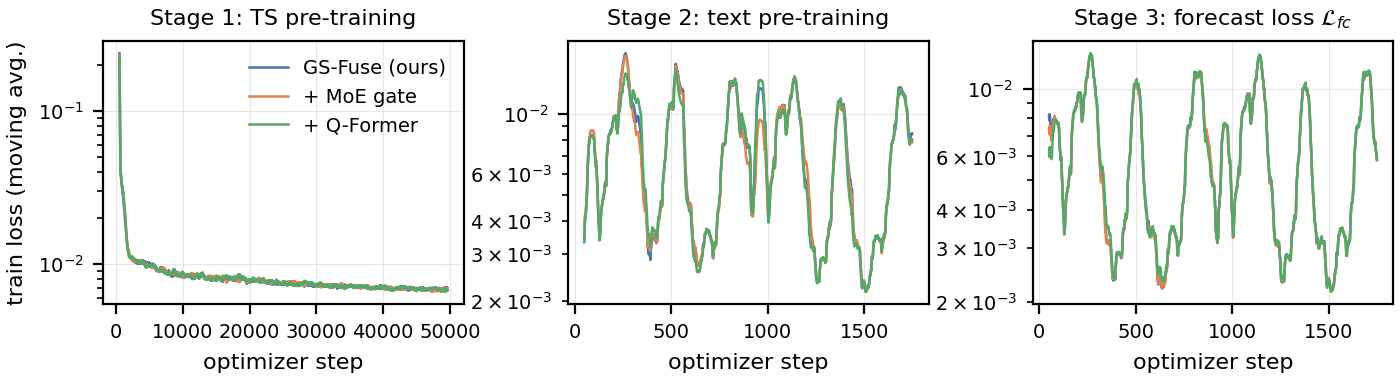
\includegraphics[width=0.9\linewidth]{figures/training_curves.png}
\caption{Our training curves for the three variants (moving average, log scale). The periodic pattern in stages 2--3 is the unshuffled, type-grouped data order repeating every epoch.}
\label{fig:curves}
\end{figure}

\subsection{Results}
\begin{table}[t]
\caption{Test MSE ($\times10^{-4}$, normalized space), endpoint DHR on close (\%), and validation MSE at $H=140$. Best model value in bold.}
\label{tab:main}
\centering\small
\begin{tabular}{l ccc ccc c}
\toprule
& \multicolumn{3}{c}{Test MSE} & \multicolumn{3}{c}{Test DHR (\%)} & Vali MSE \\
\cmidrule(lr){2-4}\cmidrule(lr){5-7}\cmidrule(lr){8-8}
Model & $H$=35 & 70 & 140 & 35 & 70 & 140 & 140 \\
\midrule
Persistence & 3.12 & 3.77 & 6.46 & -- & -- & -- & 5.94 \\
Always up & -- & -- & -- & 53.7 & 53.9 & 56.5 & -- \\
Team run & 3.36 & 3.98 & 6.66 & -- & -- & -- & 6.21 \\
\midrule
GS-Fuse (ours) & 3.05 & 3.66 & 6.33 & 54.3 & \textbf{53.0} & \textbf{54.8} & \textbf{5.80} \\
+ MoE gate & \textbf{3.03} & \textbf{3.65} & \textbf{6.32} & \textbf{54.7} & 52.6 & 54.5 & 5.81 \\
+ Q-Former & 3.06 & 3.67 & 6.33 & 53.2 & 51.7 & 54.1 & 5.83 \\
\bottomrule
\end{tabular}
\end{table}
All variants beat persistence and the team run on MSE at every horizon (Table~\ref{tab:main}). MoE is marginally best on test MSE (0.2--0.7\%) and on DHR at $H=35$; the Q-Former ties on MSE but has the lowest DHR. These gaps are below the expected seed variance, so we claim no improvement yet. Epoch 2 beat epoch 1 for every variant on validation.

\subsection{Sensitivity and ablation}
\begin{table}[t]
\caption{Modality ablation at $H=140$ (MSE $\times10^{-4}$, training-time evaluation). TS/text: only that branch kept. Text gain: test-MSE reduction of full over TS-only.}
\label{tab:abl}
\centering\small
\setlength{\tabcolsep}{4pt}
\begin{tabular}{l ccc ccc ccc}
\toprule
& \multicolumn{3}{c}{GS-Fuse (ours)} & \multicolumn{3}{c}{+ MoE gate} & \multicolumn{3}{c}{+ Q-Former} \\
\cmidrule(lr){2-4}\cmidrule(lr){5-7}\cmidrule(lr){8-10}
& full & TS & text & full & TS & text & full & TS & text \\
\midrule
Test & 6.32 & 6.35 & 6.74 & 6.31 & 6.37 & 6.80 & 6.33 & 6.42 & 9.79 \\
Vali & 5.80 & 5.86 & 6.17 & 5.81 & 5.88 & 6.17 & 5.83 & 5.92 & 9.64 \\
Text gain & \multicolumn{3}{c}{0.5\%} & \multicolumn{3}{c}{1.0\%} & \multicolumn{3}{c}{\textbf{1.4\%}} \\
$\bar\alpha_{text}$ (test) & \multicolumn{3}{c}{$0.524\pm0.003$} & \multicolumn{3}{c}{$0.522\pm0.007$} & \multicolumn{3}{c}{$0.527\pm0.006$} \\
$\mathrm{corr}(\bar\alpha_{text},\Delta)$ & \multicolumn{3}{c}{0.024} & \multicolumn{3}{c}{$-0.007$} & \multicolumn{3}{c}{\textbf{0.067}} \\
\bottomrule
\end{tabular}
\end{table}
Removing text costs the baseline 0.5\% MSE, removing prices 6\% (Table~\ref{tab:abl}). Text helps on 53\% of training samples, yet the gate is uncorrelated with when it helps (0.024): the Granger supervision is not learned. The extensions move in the intended direction: text gain rises to 1.0\% (MoE) and 1.4\% (Q-Former), and the Q-Former gate is the most correlated with the benefit (0.067). Its text-only path is far worse (9.79), so its queries are useful only together with the price context they are conditioned on.

\subsection{Error and failure case analysis}
\textbf{(1) Shrunk forecasts:} predicted close moves are only 19--34\% of the true magnitude; the MSE objective pulls forecasts toward persistence, so MAE does not improve.
\textbf{(2) Direction:} at $H=140$ the baseline predicts ``up'' for 57.3\% of events (true rate 56.5\%) and is right on 54.8\%, above the 51.0\% expected from independent signs but below always-up.
\textbf{(3) News:} 73\% of the test set is news-7/8, where MoE text openness is lowest and most variable.
\textbf{(4) Text alone} is 5--7\% worse than prices alone (baseline, MoE).

% =====================================================================
\section{Discussion: challenges and risks}\label{sec:disc}
\textbf{Leakage.} Every event is stamped at 08:30 of its date (even FOMC, released at 14:00) and news covers nearly every trading day, so 90.7\% of test and 94.1\% of validation events share an \emph{identical} input and target window with a training event. Current scores mostly measure fit to seen price paths, and duplicates inflate DHR/Sharpe significance~\cite{lopezdeprado}; this is the main correction for the final report.
\textbf{Split by type.} Validation is 96\% news-9, so model selection depends on one news stream absent from test.
\textbf{Unshuffled training} feeds one event type at a time (Figure~\ref{fig:curves}), which can bias the gate.
\textbf{Other.} All runs are single-seed; a 1B LLM may carry less signal; and the ``fine-tune the LLM's last layer'' option has no effect because the encoder runs under \texttt{no\_grad}, so the text backbone is frozen in every run, including the original code.

% =====================================================================
\section{Future directions}
\textbf{(1) Leakage-free protocol.} Use the loader's chronological split, deduplicate events sharing a window, shuffle batches, and rerun all variants with 3 seeds, a DLinear~\cite{dlinear} control, and the team's stride and 3B encoder. Everything below assumes this split; otherwise retrieval or analog memory would simply recall duplicated test windows.

\textbf{(2) Surprise-gated episodic memory from neuroscience.} Complementary learning systems theory~\cite{cls} says a slow neocortical learner (our frozen MOMENT/LLM weights) should be paired with a fast hippocampal store of specific episodes. Hippocampal prediction errors disrupt ongoing representations and, via cholinergic/dopaminergic neuromodulation, \emph{gate} whether a memory is preserved or updated~\cite{sinclair2021,neuromod}. Three-factor synaptic rules make the same idea computational: pre- and post-synaptic activity change a weight only when a surprise/neuromodulator is present~\cite{threefactor}. We will add a non-differentiable bank of $(\text{report embedding}, \text{market state}, \text{realized reaction})$ from strictly earlier dates, read by $k$NN attention~\cite{memorizing} or a modern Hopfield layer~\cite{hopfield} and written in proportion to forecast error, as in Titans~\cite{titans}. The same retrieval idea already helps in biology (AlphaFold's MSA ``memory''~\cite{alphafold}; Hopfield immune-repertoire models~\cite{deeprc}) and in forecasting (RAF~\cite{raf}, RATD~\cite{ratd}). \emph{Expected gain:} analogous past CPI/FOMC days should make $\bar\alpha_{text}$ event-specific and raise $\mathrm{corr}(\bar\alpha_{text},\Delta)$.

\textbf{(3) Memristor analog experts.} A memristor's conductance is a physical short-term memory: it depends on the recent voltage history, exactly the role of a temporal expert. Dynamic $\mathrm{WO}_x$ memristor arrays already implement reservoir computing for spoken-digit recognition and chaotic forecasting, training only a linear readout~\cite{du2017,moon2019}. Later work showed that two Ta$_2$O$_5$ devices with \emph{different forgetting time constants} $\tau$ suffice for accurate time-series prediction, and that $\tau$ can be voltage-tuned from kHz to MHz~\cite{torok2023}. Our MoE layer maps onto this hardware almost directly: each expert $E_k$ is a memristor channel (or a small reservoir) with its own $\tau_k$ (fast experts for news shocks, slow ones for payrolls/GDP), and the Granger gate is the neuromodulatory third factor that raises write current when $\Delta$ is large. \emph{Expected gain:} (i)~event-type specialization that our digital MoE almost learned but did not convert into different text weights; (ii)~orders-of-magnitude lower energy than GPU cross-attention over 1k text tokens; (iii)~a test of whether analog fading memory, rather than more transformer capacity, is what the gate is missing.

\textbf{(4) Volatility-conditioned gate and query diversity.} Feed realized volatility of $X$ and an event-type embedding to the digital gate/router, and add a query-diversity term plus a padding mask to the Q-Former. Success metric: $\mathrm{corr}(\bar\alpha_{text},\Delta)$ and per-type text gain, not only MSE.

% =====================================================================
\section{Conclusion}
We reproduced GS-Fuse at full scale, made training about 5$\times$ cheaper, and added MoE-gate and Q-Former fusion. All models beat persistence and an independent reproduction on MSE, but the gate barely uses text; the Q-Former raises the text gain from 0.5\% to 1.4\% without lowering overall error, and the released split lets most test windows appear in training. The final report will rerun all variants under a chronological, deduplicated split, which is also the prerequisite for surprise-gated memory and for testing memristor-style analog experts.

% =====================================================================
\section*{Bonus: visualization}
\begin{figure}[h]
\centering
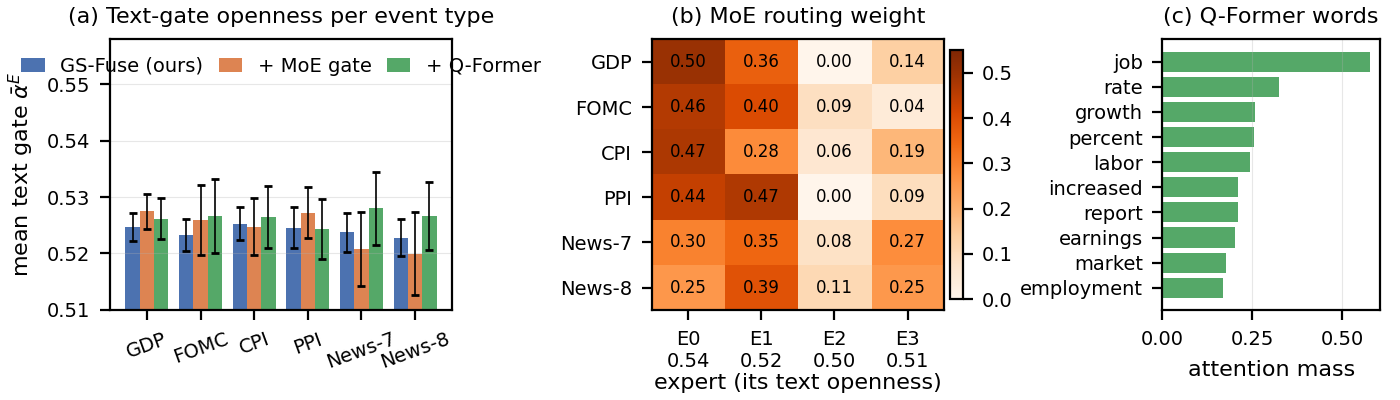
\includegraphics[width=\linewidth]{figures/interpretability.png}
\caption{(a) Mean text-gate openness per test event type (200 events, std bars). (b) MoE routing weight per event type and each expert's text openness. (c) Content words receiving the most Q-Former attention.}
\label{fig:interp}
\end{figure}
(a) Baseline text openness varies by less than 0.003 across event types. (b) The MoE router specializes (official releases go mostly to E0/E1; news uses E3 about twice as often), but all experts open the text gate to almost the same degree (0.50--0.54). (c) After removing stop-words, the Q-Former attends to macro terms (\emph{job, rate, growth, percent, labor}), but 34\% of its attention falls on padding and its 16 queries attend to nearly the same words. Details: \texttt{docs/INTERPRETABILITY.md} in our repository.

\section*{Team contributions and code}
\textbf{[Member 1]}: cloud setup, text-embedding cache, full runs, W\&B logging, evaluation and analysis.
\textbf{[Member 2]}: independent baseline run and stage-wise diagnostics.
\textbf{[Member 3]}: MoE gate and Q-Former implementation.
\textbf{[Member 4]}: related work, metrics and report.
Code: \url{https://github.com/DaezeI/11785-GS-Fuse} (branch \texttt{feat/moe-qformer-wandb-cache}).

% =====================================================================
\small
\begin{thebibliography}{99}

\bibitem{gsfuse}
Y.~Zhang, E.~Chun, Z.~Mao, Y.~Wu, and J.~Wang.
\newblock {GS-Fuse}: Granger-supervised gated fusion and multi-granularity alignment for event-driven financial forecasting.
\newblock In \emph{Proceedings of the 32nd ACM SIGKDD Conference on Knowledge Discovery and Data Mining V.2}, pages 6570--6581, 2026. doi:10.1145/3770855.3817927.

\bibitem{camef}
Y.~Zhang, W.~Yang, J.~Wang, Q.~Ma, and J.~Xiong.
\newblock {CAMEF}: Causal-augmented multi-modality event-driven financial forecasting by integrating time series patterns and salient macroeconomic announcements.
\newblock In \emph{Proceedings of the 31st ACM SIGKDD Conference on Knowledge Discovery and Data Mining V.2}, 2025. doi:10.1145/3711896.3736872.

\bibitem{moment}
M.~Goswami, K.~Szafer, A.~Choudhry, Y.~Cai, S.~Li, and A.~Dubrawski.
\newblock {MOMENT}: A family of open time-series foundation models.
\newblock In \emph{International Conference on Machine Learning (ICML)}, 2024.

\bibitem{llama3}
A.~Grattafiori et~al.
\newblock The {Llama} 3 herd of models.
\newblock \emph{arXiv preprint arXiv:2407.21783}, 2024.

\bibitem{cpc}
A.~van~den Oord, Y.~Li, and O.~Vinyals.
\newblock Representation learning with contrastive predictive coding.
\newblock \emph{arXiv preprint arXiv:1807.03748}, 2018.

\bibitem{granger}
C.~W.~J. Granger.
\newblock Investigating causal relations by econometric models and cross-spectral methods.
\newblock \emph{Econometrica}, 37(3):424--438, 1969.

\bibitem{timellm}
M.~Jin, S.~Wang, L.~Ma, Z.~Chu, J.~Y. Zhang, X.~Shi, P.-Y. Chen, Y.~Liang, Y.-F. Li, S.~Pan, and Q.~Wen.
\newblock {Time-LLM}: Time series forecasting by reprogramming large language models.
\newblock In \emph{International Conference on Learning Representations (ICLR)}, 2024.

\bibitem{timecma}
C.~Liu, Q.~Xu, H.~Miao, S.~Yang, L.~Zhang, C.~Long, Z.~Li, and R.~Zhao.
\newblock {TimeCMA}: Towards {LLM}-empowered multivariate time series forecasting via cross-modality alignment.
\newblock In \emph{AAAI Conference on Artificial Intelligence}, 2025.

\bibitem{shazeer2017}
N.~Shazeer, A.~Mirhoseini, K.~Maziarz, A.~Davis, Q.~Le, G.~Hinton, and J.~Dean.
\newblock Outrageously large neural networks: The sparsely-gated mixture-of-experts layer.
\newblock In \emph{International Conference on Learning Representations (ICLR)}, 2017.

\bibitem{switch}
W.~Fedus, B.~Zoph, and N.~Shazeer.
\newblock Switch transformers: Scaling to trillion parameter models with simple and efficient sparsity.
\newblock \emph{Journal of Machine Learning Research}, 23(120):1--39, 2022.

\bibitem{blip2}
J.~Li, D.~Li, S.~Savarese, and S.~Hoi.
\newblock {BLIP-2}: Bootstrapping language-image pre-training with frozen image encoders and large language models.
\newblock In \emph{International Conference on Machine Learning (ICML)}, 2023.

\bibitem{hyndman}
R.~J. Hyndman and A.~B. Koehler.
\newblock Another look at measures of forecast accuracy.
\newblock \emph{International Journal of Forecasting}, 22(4):679--688, 2006.

\bibitem{pesaran}
M.~H. Pesaran and A.~Timmermann.
\newblock A simple nonparametric test of predictive performance.
\newblock \emph{Journal of Business \& Economic Statistics}, 10(4):461--465, 1992.

\bibitem{fama}
E.~F. Fama.
\newblock Efficient capital markets: A review of theory and empirical work.
\newblock \emph{Journal of Finance}, 25(2):383--417, 1970.

\bibitem{dlinear}
A.~Zeng, M.~Chen, L.~Zhang, and Q.~Xu.
\newblock Are transformers effective for time series forecasting?
\newblock In \emph{AAAI Conference on Artificial Intelligence}, 2023.

\bibitem{facenet}
F.~Schroff, D.~Kalenichenko, and J.~Philbin.
\newblock {FaceNet}: A unified embedding for face recognition and clustering.
\newblock In \emph{IEEE Conference on Computer Vision and Pattern Recognition (CVPR)}, 2015.

\bibitem{adamw}
I.~Loshchilov and F.~Hutter.
\newblock Decoupled weight decay regularization.
\newblock In \emph{International Conference on Learning Representations (ICLR)}, 2019.

\bibitem{sharpe}
W.~F. Sharpe.
\newblock The {Sharpe} ratio.
\newblock \emph{Journal of Portfolio Management}, 21(1):49--58, 1994.

\bibitem{lopezdeprado}
D.~H. Bailey and M.~L{\'o}pez de Prado.
\newblock The deflated {Sharpe} ratio: Correcting for selection bias, backtest overfitting, and non-normality.
\newblock \emph{Journal of Portfolio Management}, 40(5):94--107, 2014.

\bibitem{cls}
D.~Kumaran, D.~Hassabis, and J.~L. McClelland.
\newblock What learning systems do intelligent agents need? {C}omplementary learning systems theory updated.
\newblock \emph{Trends in Cognitive Sciences}, 20(7):512--534, 2016.

\bibitem{memorizing}
Y.~Wu, M.~N. Rabe, D.~Hutchins, and C.~Szegedy.
\newblock Memorizing transformers.
\newblock In \emph{International Conference on Learning Representations (ICLR)}, 2022.

\bibitem{hopfield}
H.~Ramsauer, B.~Sch{\"a}fl, J.~Lehner, P.~Seidl, M.~Widrich, T.~Adler, L.~Gruber, M.~Holzleitner, M.~Pavlovi{\'c}, G.~K. Sandve, V.~Greiff, D.~Kreil, M.~Kopp, G.~Klambauer, J.~Brandstetter, and S.~Hochreiter.
\newblock Hopfield networks is all you need.
\newblock In \emph{International Conference on Learning Representations (ICLR)}, 2021.

\bibitem{titans}
A.~Behrouz, P.~Zhong, and V.~Mirrokni.
\newblock Titans: Learning to memorize at test time.
\newblock In \emph{Advances in Neural Information Processing Systems (NeurIPS)}, 2025. arXiv:2501.00663.

\bibitem{alphafold}
J.~Jumper et~al.
\newblock Highly accurate protein structure prediction with {AlphaFold}.
\newblock \emph{Nature}, 596:583--589, 2021.

\bibitem{deeprc}
M.~Widrich, B.~Sch{\"a}fl, M.~Pavlovi{\'c}, H.~Ramsauer, L.~Gruber, M.~Holzleitner, J.~Brandstetter, G.~K. Sandve, V.~Greiff, S.~Hochreiter, and G.~Klambauer.
\newblock Modern {Hopfield} networks and attention for immune repertoire classification.
\newblock In \emph{Advances in Neural Information Processing Systems (NeurIPS)}, 2020.

\bibitem{raf}
K.~Tire, E.~O. Taga, M.~E. Ildiz, and S.~Oymak.
\newblock Retrieval augmented time series forecasting.
\newblock \emph{arXiv preprint arXiv:2411.08249}, 2024.

\bibitem{ratd}
J.~Liu, L.~Yang, H.~Li, and S.~Hong.
\newblock Retrieval-augmented diffusion models for time series forecasting.
\newblock In \emph{Advances in Neural Information Processing Systems (NeurIPS)}, 2024.

\bibitem{sinclair2021}
A.~H. Sinclair, G.~Manalili, I.~C. Brunec, R.~A. Adcock, and M.~Barense.
\newblock Prediction errors disrupt hippocampal representations and update episodic memories.
\newblock \emph{Proceedings of the National Academy of Sciences}, 118(51):e2117625118, 2021.

\bibitem{neuromod}
T.~Palacios-Filardo and J.~R. Mellor.
\newblock Neuromodulation of hippocampal long-term synaptic plasticity.
\newblock \emph{Current Opinion in Neurobiology}, 54:37--43, 2019.

\bibitem{threefactor}
N.~Fr{\'e}maux and W.~Gerstner.
\newblock Neuromodulated spike-timing-dependent plasticity, and theory of three-factor learning rules.
\newblock \emph{Frontiers in Neural Circuits}, 9:85, 2016.

\bibitem{du2017}
C.~Du, F.~Cai, M.~A. Zidan, W.~Ma, S.~H. Lee, and W.~D. Lu.
\newblock Reservoir computing using dynamic memristors for temporal information processing.
\newblock \emph{Nature Communications}, 8:2204, 2017.

\bibitem{moon2019}
J.~Moon, W.~Ma, J.~H. Shin, F.~Cai, C.~Du, S.~H. Lee, and W.~D. Lu.
\newblock Temporal data classification and forecasting using a memristor-based reservoir computing system.
\newblock \emph{Nature Electronics}, 2:480--487, 2019.

\bibitem{torok2023}
D.~Moln{\'a}r, T.~N.~T{\"o}r{\"o}k, J.~Volk, Z.~Balogh, and A.~Halbritter.
\newblock Neural information processing and time-series prediction with only two dynamical memristors.
\newblock \emph{arXiv preprint arXiv:2307.13320}, 2023.

\end{thebibliography}

\end{document}
